\chapter{AMG Solver}

If $A$ is a positive-definite square matrix, the AMG methods
\cite{AMG, AMG-OR, Stuben2, BMR, falgout, psm} have proved to be
efficient methods and they are also scalable \cite{rsamg}.

AMG methods have hierarchical structures, which is shown in Figure \ref{fig-amg}.
A coarse grid is constructed when entering a coarser level.
To calculate a coarser matrix, a restriction operator $R_l$ and
an interpolation (prolongation) operator $P_l$ need to be determined.
In general, the restriction operator $R_l$ is the transpose of the interpolation (prolongation) operator $P_l$:

\[
R_l = P_l^T.
\]
The matrix on the coarser grid is calculated as
\begin{equation}
A_{l + 1} = R_l A_l P_l.
\end{equation}
We know that a high frequency error is easier to converge on a fine grid than a low frequency error, and
for the AMG methods,
the restriction operator, $R_l$, projects the error from a finer grid onto a coarser grid and
converts a low frequency error to a high frequency error.
The interpolation operator transfers a solution on a coarser
grid to that on a finer grid.
Its setup phase for the AMG methods on each level $l$ ($0 \leq l < L$) is formulated in
Algorithm \ref{alg-amg-setup}, where a coarser grid, an interpolation operator, a restriction
operator, a coarser matrix and post- and pre-smoothers are constructed.
By repeating the algorithm, an $L$-level system can be built.
The solution of the AMG methods is recursive and is formulated in Algorithm \ref{alg-amg-solve}, which
shows one iteration of AMG.

\begin{figure}[!htb]
    \centering
    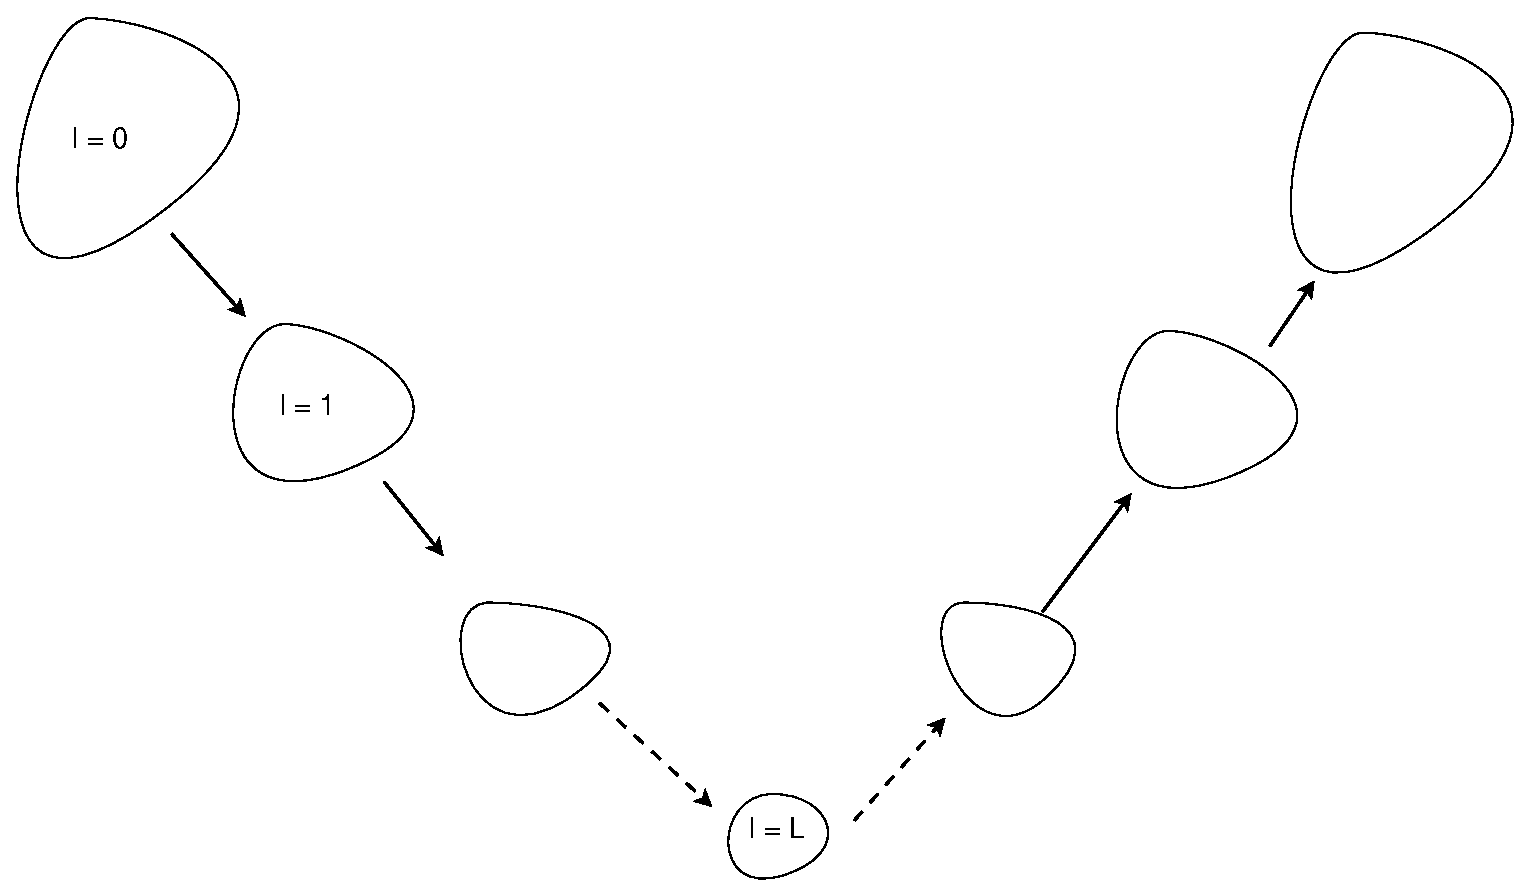
\includegraphics[width=0.650\linewidth]{amg}
    \caption{Structure of AMG solver.}
    \label{fig-amg}
\end{figure}

\begin{algorithm}[!htb]
\caption{AMG setup Algorithm} \label{alg-amg-setup}
\begin{algorithmic}[1]
  \State Calculate strength matrix $S$.
  \State Choose coarsening nodes set $\omega_{l+1}$ according to strength matrix $S$, such that $\omega_{l+1} \subset \omega_{l}$.
  \State Calculate prolongation operator $P_l$.
  \State Derive restriction operator $R_l = P_l^T$.
  \State Calculate coarse matrix $A_{l+1}$: $A_{l+1} = R_l \times A_l \times P_l$.
  \State Setup pre-smoother $S_l$ and post-smoother $T_l$.
\end{algorithmic}
\end{algorithm}

\begin{algorithm}[!htb]
\caption{AMG V-cycle Solution Algorithm: amg\_solve($l$)} \label{alg-amg-solve}
\begin{algorithmic}%[1]
\State Require: $b_l$, $x_l$, $A_l$, $R_l$, $P_l$, $S_l$, $T_l$, $0 \leq l < L$
\State
\State $b_0 = b$

\If {($l < L$)}
  \State $x_l = S_l(x_l, A_l, b_l)$
  \State $r = b_l - A_lx_l$
  \State $b_{r+1} = R_lr$
  \State amg\_solve($l+1$)
  \State $x_l = x_l + P_l x_{l+1}$
  \State $x_l = T_l(x_l, A_l, b_l)$
\Else
  \State $x_l = A_l^{-1}b_l$
\EndIf

\State x = $x_0$

\end{algorithmic}
\end{algorithm}

The Cleary-Luby-Jones-Plassman (CLJP) coarsening
algorithm was proposed by Cleary \cite{cljp1} based on the algorithms developed
by Luby \cite{cljp3} and Jones and Plassman \cite{cljp2}. The standard RS coarsening algorithm
has also been parallelized \cite{HYPRE2}. Falgout et al. developed a parallel coarsening algorithm,
the Falgout coarsening algorithm, which has been implemented in HYPRE \cite{HYPRE2}. Yang et al. proposed
HMIS and PMIS coarsening algorithms for a coarse grid selection \cite{pmis}. Various parallel smoothers
and interpolation operators have also been studied by Yang et al \cite{HYPRE2,pmis}.

\section{Data Structures}

\nverb{SX_SM_TYPE} defines smoother types. The following smoothers are implemented,
\begin{evb}
typedef enum
{
    SX_SM_JACOBI    = 1,  /**< Jacobi smoother */
    SX_SM_GS        = 2,  /**< Gauss-Seidel smoother */
    SX_SM_SGS       = 3,  /**< Symmetric Gauss-Seidel smoother */
    SX_SM_SOR       = 4,  /**< SOR smoother */
    SX_SM_SSOR      = 5,  /**< SSOR smoother */
    SX_SM_GSOR      = 6,  /**< GS + SOR smoother */
    SX_SM_SGSOR     = 7,  /**< SGS + SSOR smoother */
    SX_SM_POLY      = 8,  /**< Polynomial smoother */
    SX_SM_L1DIAG    = 9,  /**< L1 norm diagonal scaling smoother */

} SX_SM_TYPE;
\end{evb}

\nverb{SX_COARSEN_TYPE} defines coarsening types, including classical RS coarsening and
classical RS coarsening with positive off-diagonals.
\begin{evb}
typedef enum
{
    SX_COARSE_RS      = 1,  /**< Classical */
    SX_COARSE_RSP     = 2,  /**< Classical, with positive offdiags */

} SX_COARSEN_TYPE;
\end{evb}


\nverb{SX_INTERP_TYPE} defines interpolation types, including direct interpolation
and standard interpolation.
\begin{evb}
typedef enum
{
    SX_INTERP_DIR     = 1,  /**< Direct interpolation */
    SX_INTERP_STD     = 2,  /**< Standard interpolation */

} SX_INTERP_TYPE;
\end{evb}


\nverb{SX_AMG_PARS} defines AMG parameters. The meaning of each member is explained as comment. For example,
\nverb{cycle_itr}
determines the cycle type: 1 for V-cycle, 2 for W-cycle..
\begin{evb}
typedef struct SX_AMG_PARS
{
    SX_INT verb;

    SX_INT   cycle_itr;          /** type of AMG cycle, 1 is for V, W if greater than 1 */
    SX_FLOAT tol;                /** stopping tolerance for AMG solver */
    SX_FLOAT ctol;               /** stopping tolerance for coarsest solver */
    SX_INT   maxit;              /** maximal number of iterations of AMG */

    SX_COARSEN_TYPE cs_type;     /** coarsening type */
    SX_INT max_levels;           /** max number of levels of AMG */
    SX_INT coarse_dof;           /** max number of coarsest level DOF */

    SX_SM_TYPE smoother;         /** smoother type */
    SX_FLOAT   relax;            /** relax parseter for SOR smoother */
    SX_INT     cf_order;         /** False (0): nature order, True (1): C/F order */
    SX_INT     pre_iter;         /** number of presmoothers */
    SX_INT     post_iter;        /** number of postsmoothers */
    SX_INT     poly_deg;         /** degree of the polynomial smoother */

    SX_INTERP_TYPE interp_type;  /** interpolation type */
    SX_FLOAT strong_threshold;   /** strong connection threshold for coarsening */
    SX_FLOAT max_row_sum;        /** maximal row sum parseter */
    SX_FLOAT trunc_threshold;    /** truncation threshold */

} SX_AMG_PARS;
\end{evb}

\nverb{SX_RTN} is for return values.
\begin{evb}
typedef struct SX_RTN
{
    SX_FLOAT ares;     /* absolute residual */
    SX_FLOAT rres;     /* relative residual */
    SX_INT   nits;     /* number of iterations */

} SX_RTN;
\end{evb}

\section{Management}

\subsection{Initialize Parameters}

\nverb{sx_amg_pars_init} sets default parameters.
\begin{evb}
void sx_amg_pars_init(SX_AMG_PARS *pars);
\end{evb}

\subsection{Setup}
\nverb{sx_amg_setup} setups the hierarchical struture of AMG solver using given parameters.
\begin{evb}
SX_AMG * sx_amg_setup(SX_MAT *A, SX_AMG_PARS *pars);
\end{evb}

\subsection{Solve}

\nverb{sx_solver_amg_solve} solves the linear system using AMG method. The AMG object has to be
set up before using, the \nverb{x} has initial value and \nverb{b} is the right-hand side.
\begin{evb}
SX_RTN sx_solver_amg_solve(SX_AMG *mg, SX_VEC *x, SX_VEC *b);
\end{evb}

\nverb{sx_solver_amg} solves the linear system using AMG method. This function is a high level 
interface, and user can call it to solve a linear system, which will setup the AMG object,
solve and destroy the AMG object. If \nverb{pars} is \verb|NULL|, then default parameters
will be applied.
\begin{evb}
SX_RTN sx_solver_amg(SX_MAT *A, SX_VEC *x, SX_VEC *b, SX_AMG_PARS *pars);
\end{evb}

\subsection{Destroy}
\nverb{sx_amg_data_destroy} destroys the AMG object.
\begin{evb}
void sx_amg_data_destroy(SX_AMG **mg);
\end{evb}

